% 
\section{Benchmark Evaluation}
\label{sec:exp}

In this section, we present our comprehensive evaluation of state-of-the-art monocular deep visual SLAM systems, designed to test their limits on ScaleMaster benchmark. Our complete experimental workflow—from data acquisition with our custom rig, through metric SE(3) pose estimation and baseline metric map generation, to the final map-to-map error calculation—is illustrated in \figref{fig:system_overview}. 

Our analysis proceeds in three stages: we begin by applying conventional trajectory metrics to uncover Sim(3) pose estimation failure cases, then demonstrate the inherent limitations of relying on these metrics alone, and finally introduce our direct map-to-map quality evaluation \cite{wu2021density}, which provides evidence of geometric inconsistencies further supported by qualitative visualizations.

% 
\subsection{Experimental Setup}
\label{sec:exp-setup}

% 
\begin{itemize}
  \item \textbf{Baselines:} 
  We evaluate three representative deep learning-based SLAM systems: \text{DROID-SLAM} \cite{teed2021droid}, \text{MASt3R-SLAM} \cite{murai2025mast3r}, and \text{VGGT-SLAM} \cite{maggio2025vggt}. All experiments were conducted using the official implementations provided by the authors, on a desktop with an AMD Ryzen 9 9900X CPU and an NVIDIA RTX 5090 GPU.
  
  \item \textbf{(Pose-oriented) Trajectory Evaluation:} 
  All trajectories are evaluated using the \ac{ATE} in \ac{RMSE} (m) using the \texttt{evo} evaluator \cite{grupp2017evo}. To ensure comparability, a $\text{Sim}(3)$ alignment \cite{umeyama2002least} was applied for scale correction because our primary focus is on intra- and inter-scale consistency challenges, rather than on metric scale evaluation (i.e., a single global scale parameter estimation).
  
  \item \textbf{(Map-oriented) 3D Reconstruction Quality Evaluation:} 
  We assess geometric fidelity by aligning the SLAM-generated map to a LiDAR point cloud, which we treat as a near–ground-truth metric map. We apply the scale, rotation, and translation $(s,R,t)$ parameters derived from the aforementioned \texttt{evo} trajectory alignment based on Umeyama algorithm. This method tests the hypothesis that a correct trajectory should yield a correct map under the same transformation. After alignment, we compute the Chamfer distance and the Drop Rate(\%); we define the Drop Rate as the percentage of points in the SLAM-generated map that have no corresponding point in the ground truth metric map within a predefined distance threshold. This metric is designed to quantify severe outliers and regions of complete map failure.
\end{itemize}

% 
\subsection{Trajectory Evaluation}
\label{sec:exp-quant}

We begin our quantitative analysis with the standard \ac{ATE} to first establish a performance baseline and then reveal the critical failure modes that our benchmark uniquely exposes. As shown in  \tabref{arkit}, leading algorithms like MASt3R-SLAM reconfirm their state-of-the-art performance on the ARKitScenes dataset \cite{dehghan2021arkitscenes}, which establishes a baseline of their high performance under controlled, small-sized room conditions. This result can overstate general robustness.
However, this perception of robustness does not hold when evaluated on the targeted challenges of our ScaleMaster dataset, as detailed in \tabref{tab:benchmark_our}. For instance, in long-range sequences like \texttt{LargeHall\_01}, the trajectory error surges to the 80-90 meter range. This is not a random tracking loss but a direct consequence of accumulated scale drift over a long trajectory. A similar phenomenon can be observed in a different sequence, as illustrated in \figref{fig:long_term_7}.

These contrasting ATE results serve as a clear numerical demonstration that an algorithm's stability can be severely compromised by the scale-related challenges present in real-world environments, a weakness that remains hidden when evaluated on simpler, less complex benchmarks.

% 
\begin{table}[t]
\centering
\caption{Absolute Trajectory Error (ATE (m)) on ARKitScenes sequences \cite{dehghan2021arkitscenes}.}
\begin{threeparttable}
\resizebox{0.75\columnwidth}{!}{%
\begin{tabular}{l|cccc}
\midrule
{\small \textbf{Sequence}} & 
\makecell{\textbf{DROID}\\\textbf{SLAM}} & 
\makecell{\textbf{VGGT}\\\textbf{SLAM}} & 
\makecell{\textbf{MASt3R}\\\textbf{SLAM}} & 
\makecell{\textbf{MASt3R}\\\textbf{SLAM*}} \\ 
\midrule
40777073  & 0.65 & 0.24 & 0.18 & \textbf{0.13} \\
40958754  & 0.20 & 0.03 & 0.09 & \textbf{0.02} \\
40958756  & 0.21 & 0.07 & 0.08 & \textbf{0.03} \\
41007589  & 0.32 & 0.05 & 0.09 & \textbf{0.03} \\
41045408  & \textbf{0.01} & 0.06 & 0.05 & \textbf{0.01} \\
41048083  & 0.77 & 0.82 & \textbf{0.08} & \textbf{0.08} \\
41048120  & 0.06 & 0.39 & 0.06 & \textbf{0.05} \\
\midrule
\textbf{Average} & 0.32 & 0.24 & 0.09 & \textbf{0.05} \\
\midrule
\end{tabular}}

\begin{tablenotes}[flush]
\item  \footnotesize * : calibrated mode
\end{tablenotes}
\end{threeparttable}

% \vspace{-5mm}

\label{arkit}
\end{table}
% 

% 
\begin{table}[t!]
\centering
\caption{Absolute Trajectory Error (unit: meter) on our dataset.}
\begin{threeparttable}
\resizebox{0.95\columnwidth}{!}{%
\begin{tabular}{l|cccc}
\midrule
{\small \textbf{Sequence}} & 
\makecell{\textbf{DROID}\\\textbf{SLAM}} & 
\makecell{\textbf{VGGT}\\\textbf{SLAM}} & 
\makecell{\textbf{MASt3R}\\\textbf{SLAM}} & 
\makecell{\textbf{MASt3R}\\\textbf{SLAM*}} \\ 
\midrule
{\footnotesize Basement\_01} &\textbf{0.08}& 1.44 & 0.38 & 0.42 \\
{\footnotesize HotelRoom\_01} & 0.05 & -- & 0.10 & \textbf{0.06} \\
{\footnotesize Lab\_01} & 0.36 & -- & 0.36 & \textbf{0.09} \\
{\footnotesize LargeHall\_01} & 89.35 & -- & \textbf{80.54} & 91.62 \\
{\footnotesize LargeHall\_02} & \textbf{3.78} & 21.69 & 6.12 & 5.89 \\
{\footnotesize LargeHall\_03} & 13.21 & -- & 1.99 & \textbf{1.96} \\
{\footnotesize LargeHall\_04} & 4.01 & 1.12 & \textbf{0.57} & 0.92 \\
{\footnotesize LargeHall\_05} & 0.56 & 0.51 & 0.45 & \textbf{0.33} \\
{\footnotesize Library\_01} & \textbf{1.68} & -- & 5.29 & 3.61 \\
{\footnotesize Library\_02} & 1.45 & -- & 0.54 & \textbf{0.63} \\
{\footnotesize Library\_03} & 0.09 & -- & 0.09 & \textbf{0.06} \\
{\footnotesize Library\_04} & 4.86 & -- & 3.54 & \textbf{3.22} \\
{\footnotesize Library\_05} & 4.35 & 13.26 & \textbf{3.08} & 4.00 \\
{\footnotesize Library\_06} & 0.05 & -- & 0.05 & \textbf{0.04} \\
{\footnotesize Library\_07} & 0.13 & 0.22 & 0.13 & \textbf{0.12} \\
{\footnotesize Library\_08} & 0.09 & -- & 0.09 & \textbf{0.06} \\
{\footnotesize Library\_09} & 0.04 & -- & 0.07 & \textbf{0.05} \\
{\footnotesize Lobby\_01} & 0.76 & 3.18 & 0.54 & \textbf{0.27} \\
{\footnotesize Lounge\_01} & 4.51 & -- & 0.47 & \textbf{0.16} \\
{\footnotesize Office\_01} & 5.61 & -- & 8.03 & \textbf{0.65} \\
{\footnotesize Parking\_01} & \textbf{10.21} & -- & 32.37 & 26.13 \\
{\footnotesize Parking\_02} & \textbf{0.20} & -- & 0.39 & 0.21 \\
{\footnotesize Stairs\_01} & 20.20 & -- & 4.60 & \textbf{2.30} \\
{\footnotesize Stairs\_02} & 5.59 & 1.05 & 1.00 & \textbf{0.14} \\
{\footnotesize Station\_01} & 11.66 & -- & 13.21 & \textbf{4.37} \\
\midrule
\end{tabular}%
} 
\vspace{2mm}
\begin{tablenotes}[flushleft]
\item \footnotesize
\parbox{0.98\columnwidth}{%
* : calibrated mode \\
-- : Runs that terminated with an invalid pose update (negative determinant during SL(4) normalization) were marked as failures; ATE is therefore undefined for those sequences.
}
\end{tablenotes}
% \vspace{-5mm}
\end{threeparttable}
\label{tab:benchmark_our}
\end{table}

% 

% 
\begin{table}[t]
\centering
\caption{3D Reconstruction Quality of MASt3R-SLAM}
\label{table:recon_quality}
\resizebox{1.0\columnwidth}{!}{%
\begin{tabular}{l|cccc}
\hline
\toprule
\makecell{\textbf{Sequence}\\\textbf{Name}} & 
\makecell{\textbf{Threshold} } & 
\makecell{\textbf{Chamfer}\\\textbf{Distance(m)}} & 
\makecell{\textbf{Drop}\\ \textbf{Rate}(\%)} & 
\textbf{Analysis} \\
\midrule
\multirow{2}{*}{\makecell[l]{\textbf{Library\_01}}}
  & 1  & 0.36 & 42.5 & \textbf{Severe Failure} \\
  & 10 & \textbf{6.43} & 0.9 & Significant map distortion. \\
\hline
\multirow{2}{*}{\textbf{Library\_06}} 
  & 1  & 0.08 & 1.1 & \textbf{Success} \\
  & 10 & \textbf{0.10} & 0.0 & High-fidelity reconstruction. \\
\hline
\multirow{2}{*}{\textbf{Library\_07}} 
  & 1  & 0.52 & \textbf{89.1} & \textbf{Catastrophic Failure} \\
  & 10 & \textbf{9.99} & 0.0 & Near-total map collapse. \\
  
\bottomrule
\hline
\end{tabular}}
% \vspace{-3mm}
\label{map_qual}
\end{table}
% 

% 
\begin{figure}[!t]
    \centering
    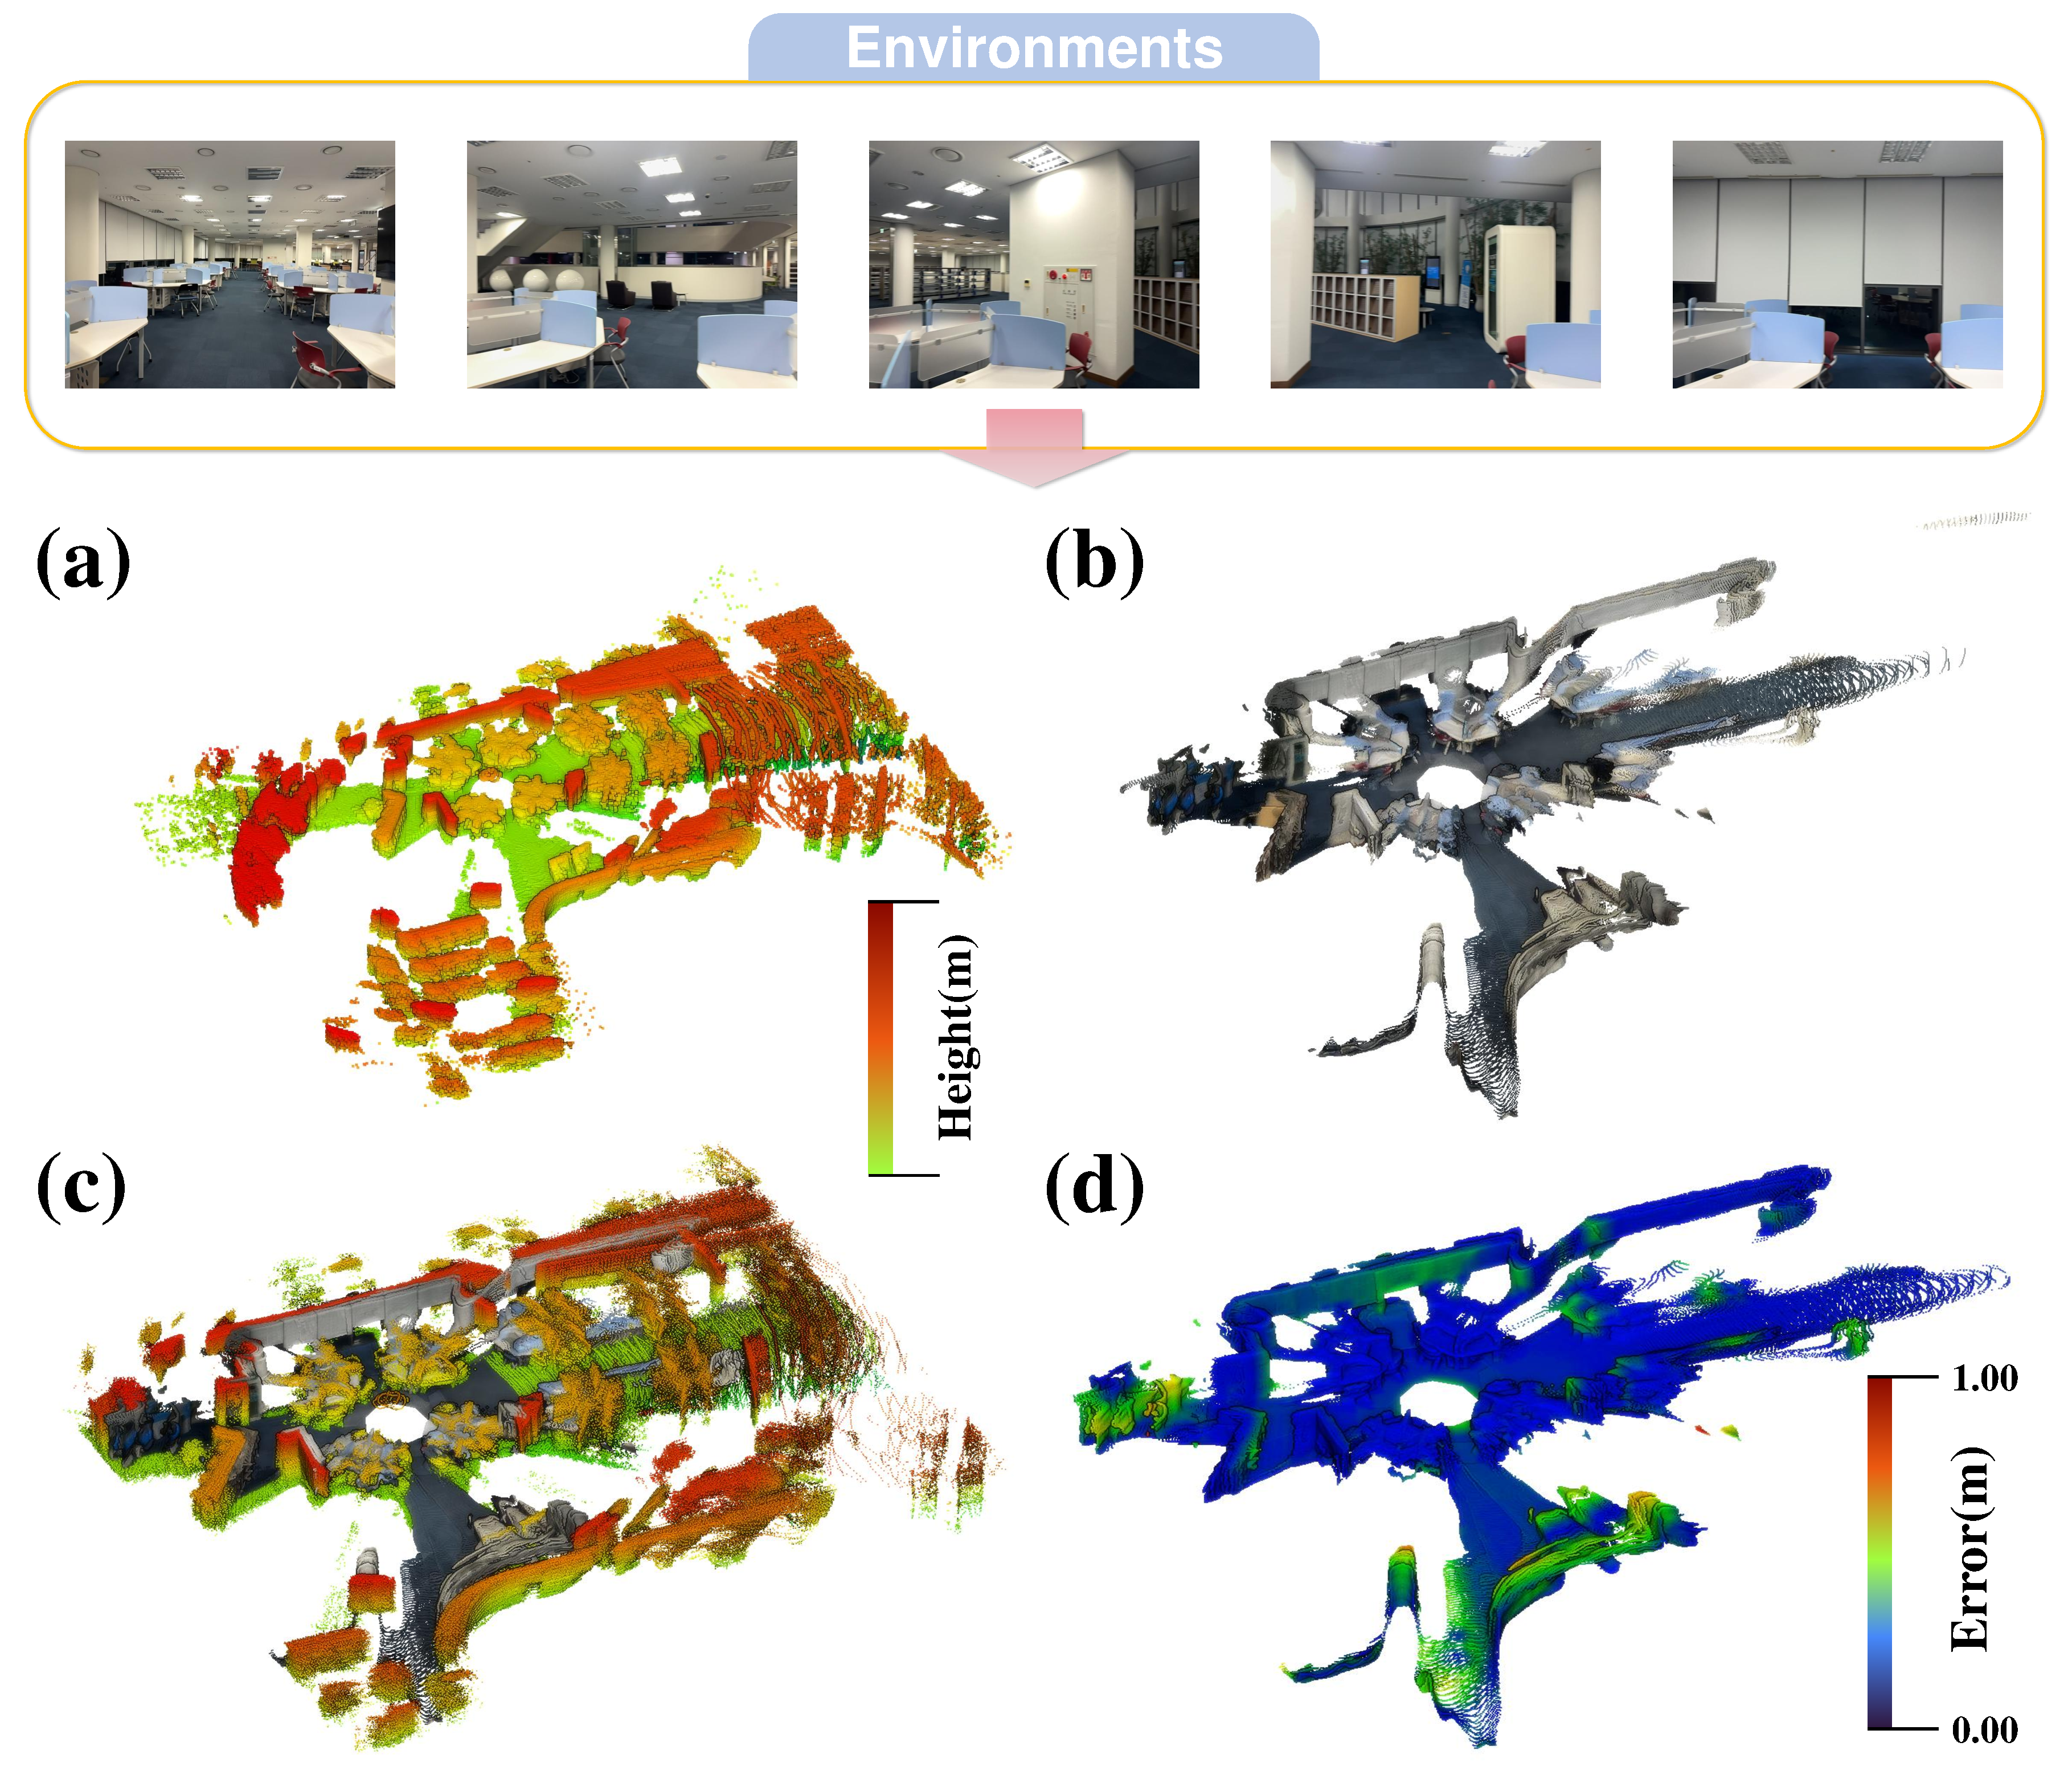
\includegraphics[width=1.0\columnwidth]{fig/fig_sample.pdf}
    \caption{Qualitative comparison of 3D reconstruction of the \texttt{Library\_06} sequence. (a) Ground truth point cloud from LiDAR, color-coded by height. (b) The map reconstructed by MASt3R-SLAM. (c) The alignment of the MASt3R-SLAM map onto the ground truth. (d) Point-to-point distance error visualization, where warmer colors (red) indicate larger geometric inconsistencies between the two maps}
    
    \vspace{-3mm}
    
    \label{fig:lib6_fig}
\end{figure}
% 

% 
\begin{figure}[t]
    \centering
    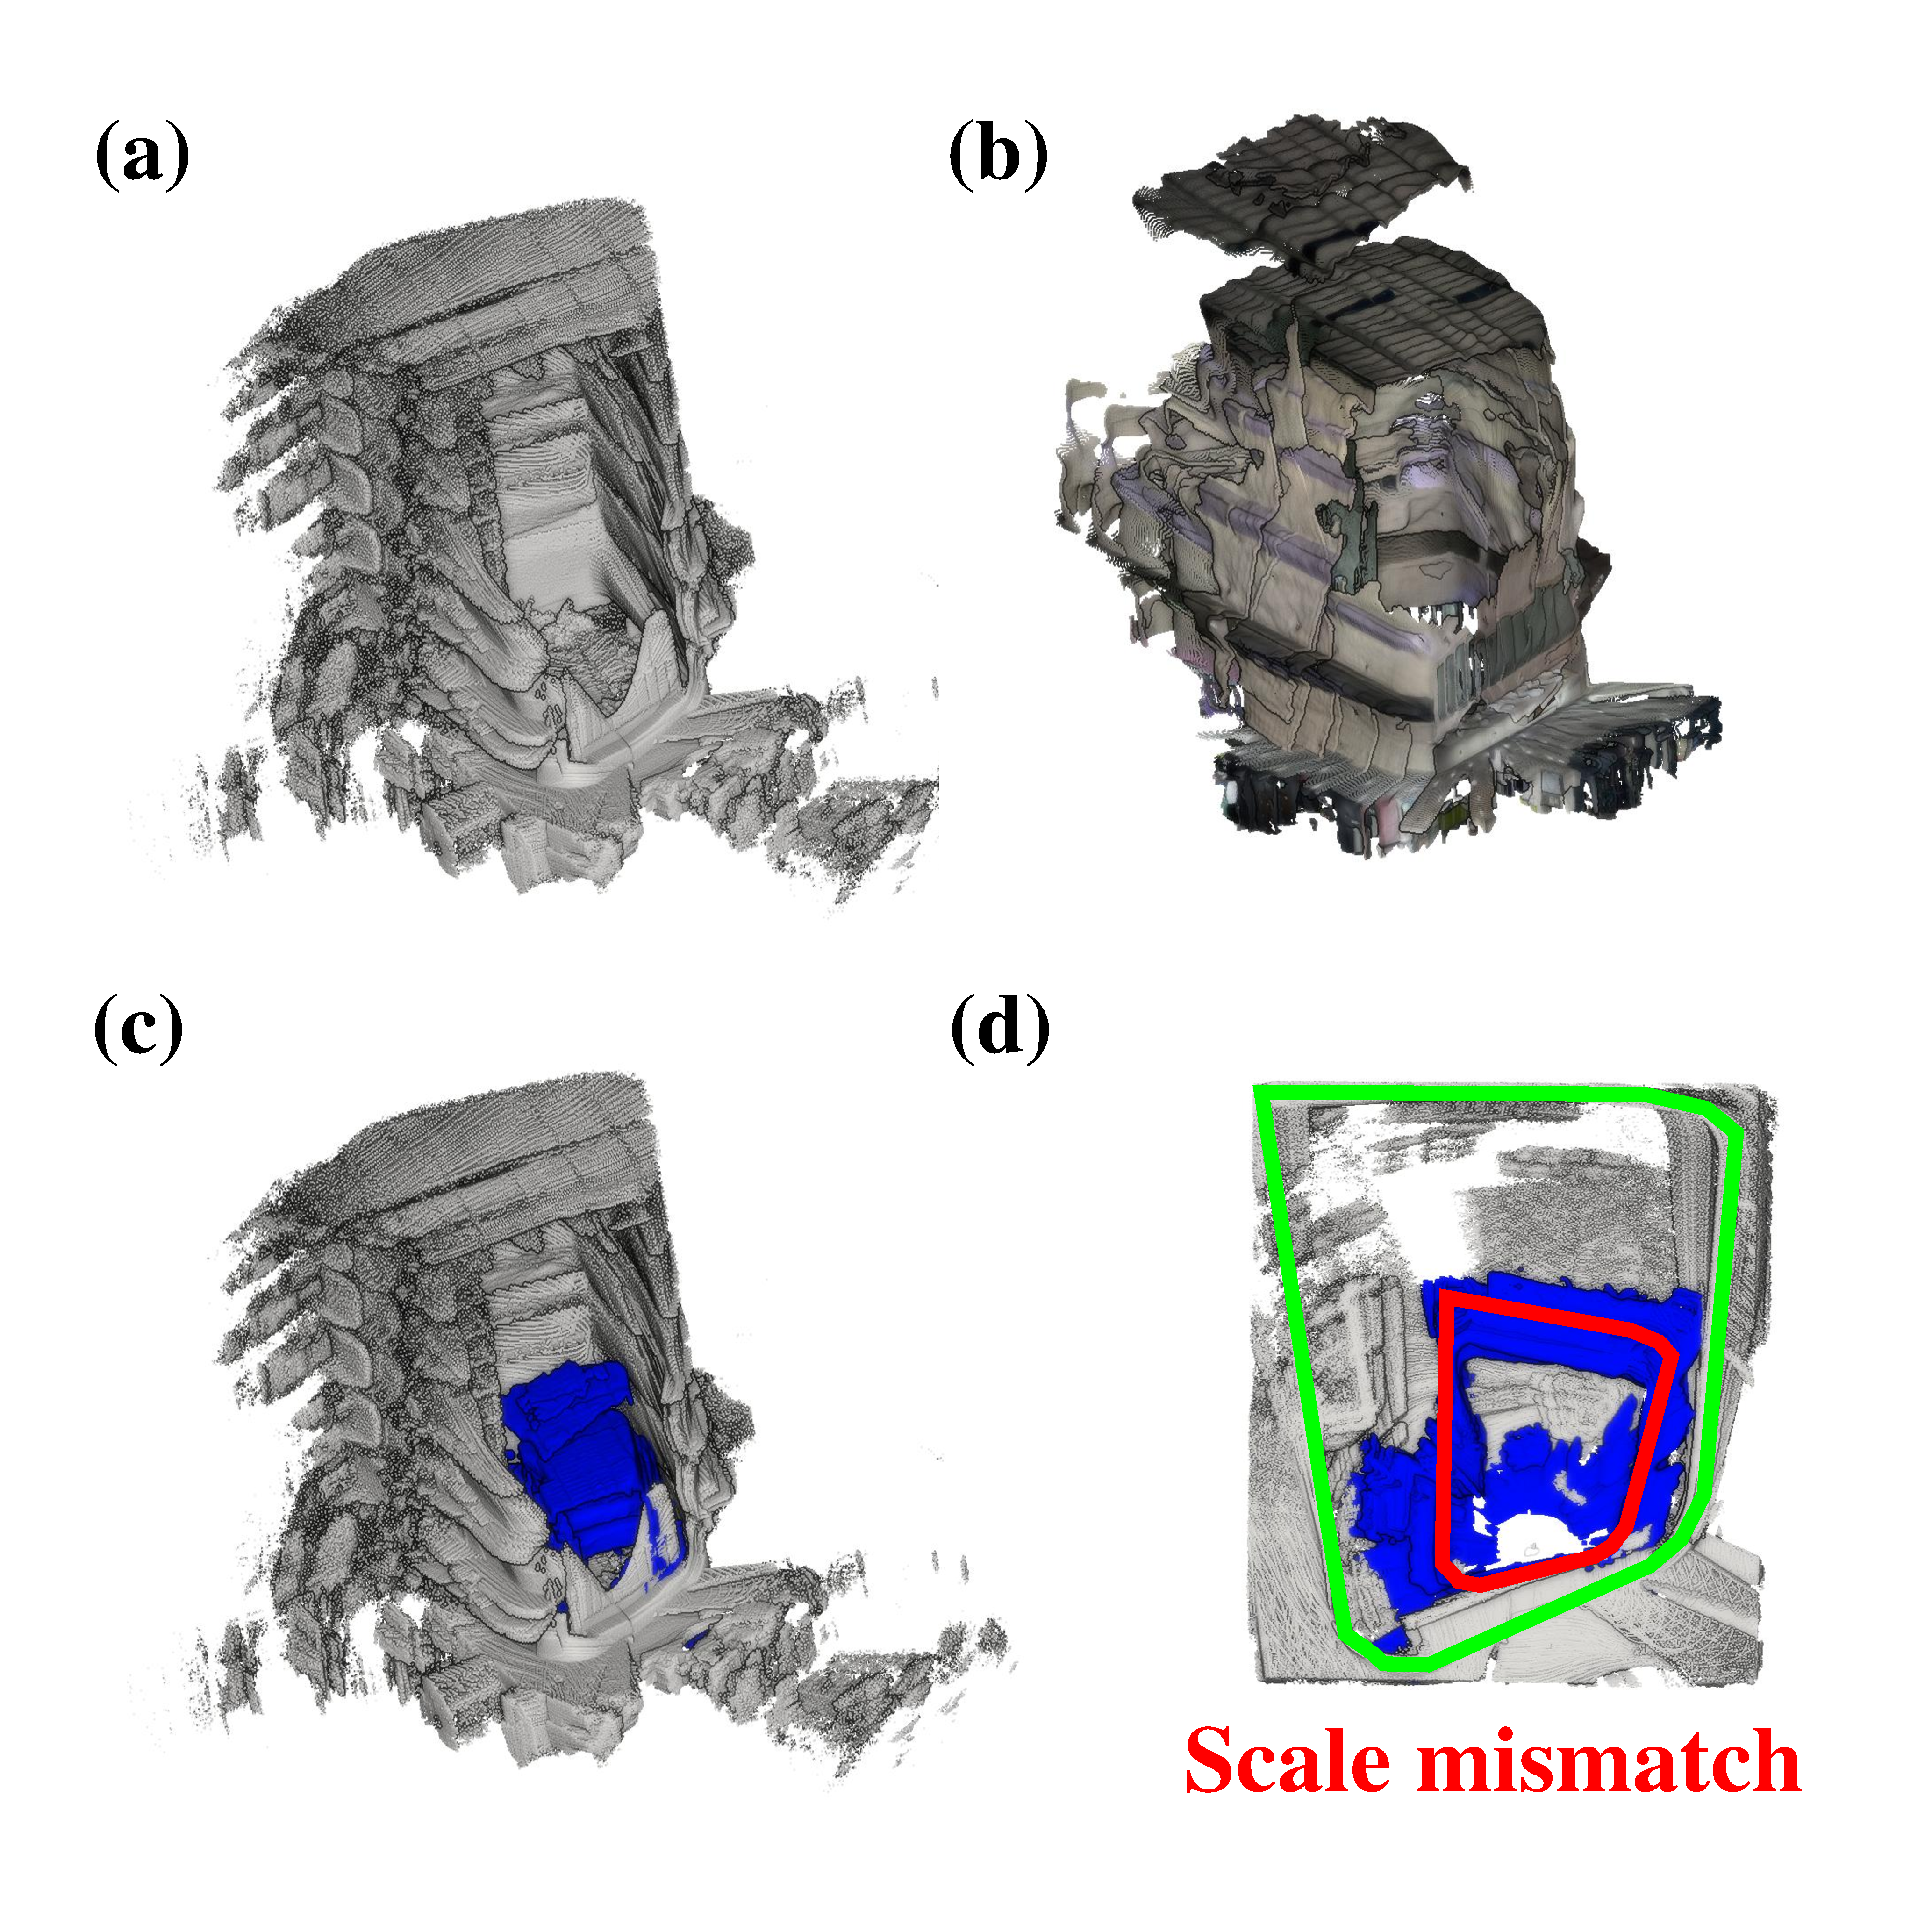
\includegraphics[width=1.0\columnwidth,height=0.3\textheight]{fig/fig5.pdf}
    \caption{Qualitative comparison on \texttt{Library\_07} demonstrating that low trajectory error does not guarantee correct map scale. (a) The LiDAR ground-truth and (b) the MASt3R-SLAM reconstruction. (c) The overlay and (d) top-down cross-section are generated after applying the single global Sim(3) transformation calculated to align the camera trajectories.}

    \vspace{-3mm}
    
    \label{fig:lib1_fig}
\end{figure}
% 

% 
\subsection{3D Reconstruction Quality: Exposing Geometric Failures}
\label{sec:exp_map}

While the dramatic \ac{ATE} failures are informative, \ac{ATE} provides only a partial characterization of system performance. It does not describe the geometric fidelity and completeness of a resulting dense 3D map, which is the primary output of a dense visual SLAM system. As our subsequent analysis will prove, a SLAM system can produce a trajectory with low ATE, yet the corresponding map can be severely warped or incorrectly scaled due to internal scale inconsistencies. Therefore, a more direct evaluation of the 3D map is essential \cite{hu2025mapeval}.

To overcome the limitations of ATE, we use Chamfer distance and Drop Rate mentioned in \secref{sec:exp-setup}. These direct map-to-map quality evaluations are presented in \tabref{map_qual}. This analysis reveals the metric reconstruction failures.

\begin{itemize}
  \item \textbf{Success Case}:
  On the \texttt{Library\_06} sequence (see \figref{fig:lib6_fig}), the baseline algorithm (e.g., MASt3R-SLAM) performs well in both pose estimation (0.04 m in \tabref{tab:benchmark_our}) and map reconstruction up to a single global scale, achieving a low Chamfer distance of 0.10 m. This example is the case where the scale is well maintained, thus both the trajectory and the map are correct.

  \item \textbf{Catastrophic Failure Case}: 
  In contrast, \figref{fig:lib1_fig} shows that the \texttt{Library\_07} sequence suffers a geometric failure even though the pose error is low (0.12 m in \tabref{tab:benchmark_our}). With the correspondence distance threshold set to 1 m, 89.1\% of the generated map points were discarded as outliers, and when the threshold was increased to 10 m, the Chamfer distance reached a massive 9.99 m. This scale consistency-aware reconstruction failure is fundamentally invisible to ATE but is captured perfectly by the map quality metrics.  
\end{itemize}
These results show that trajectory error alone, even after a single scalar scale adjustment, is insufficient and often misleading. Direct map quality evaluation is therefore necessary to assess dense visual SLAM reliably.

% 
\subsection{Qualitative Analysis of Scale Inconsistency}
\label{sec:exp_qual}

Building on the taxonomy of scale inconsistency outlined in \figref{fig:problem_diagram}, we now illustrate three representative failure cases, each corresponding to a distinct category of the problem. The following three figures (\figref{fig:short_term_scale_inconsistency}, \figref{fig:long_term_7}, and \figref{fig:multi_scale_inconsistency})  serve as visual counterparts to the taxonomy in Fig. 2, grounding the abstract categories in concrete empirical evidence.

\noindent \textbf{Intra-session Scale Inconsistency:} \figref{fig:short_term_scale_inconsistency} illustrates short-term scale failure in a vertical motion sequence, \texttt{Station\_01}. Repetitive stair patterns disrupt data association between consecutive frames, causing immediate scale drift and severe map distortions like multi-layer overlaps. Furthermore, \figref{fig:long_term_7} shows a long-term optimization failure on the \texttt{Parking\_01} sequence. Although a loop closure is detected, the massive accumulated scale drift traps the optimizer in a local minimum, resulting in a geometrically inconsistent map.

\noindent \textbf{Inter-session Scale Ambiguity:} \figref{fig:multi_scale_inconsistency} demonstrates another critical issue. When a single video is processed as three independent sessions, each resulting map fragment is generated at a different, inconsistent scale. While internally coherent, they cannot be merged into a single, globally scale-consistent map, highlighting a major challenge for long-term mapping or collaborative SLAM.   

% 
\begin{figure}[t]
    \centering
    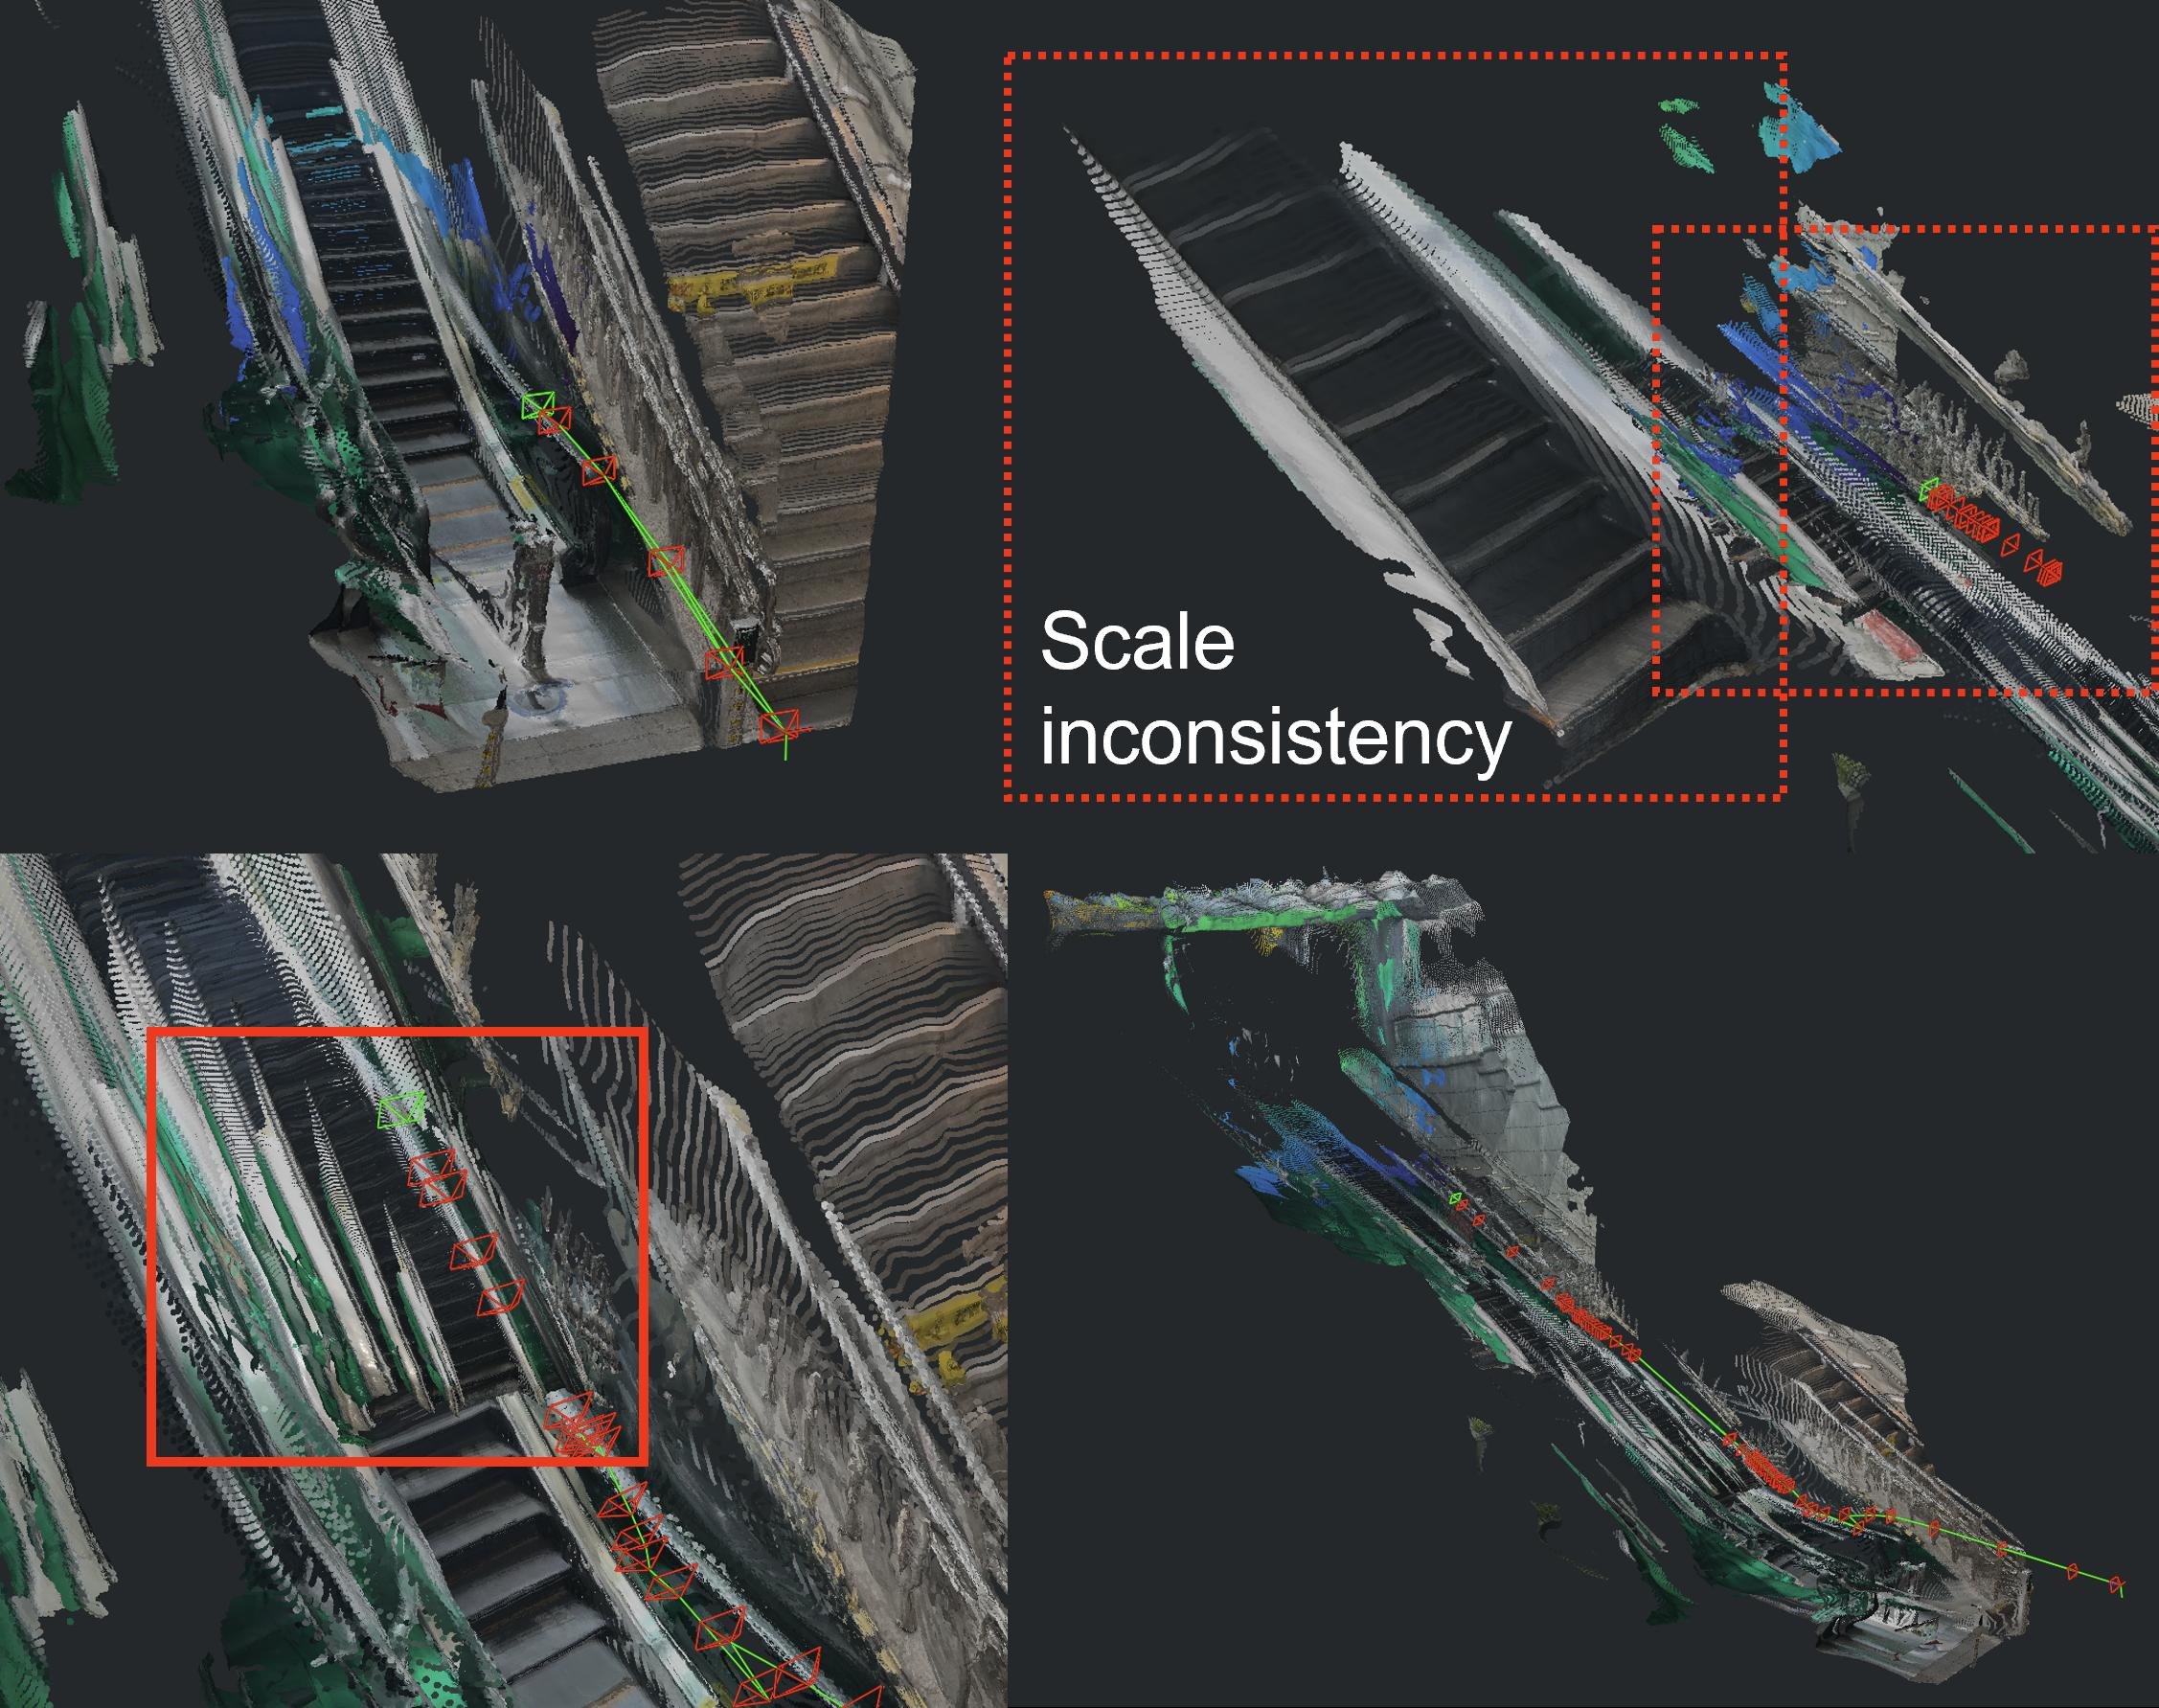
\includegraphics[width=0.95\columnwidth]{fig/short_term_scale_inconsistency_fig.jpg}
    \caption{Short-term scale inconsistency of MASt3R-SLAM on the \texttt{Station\_01} sequence. The repetitive structure and vertical motion cause a severely distorted and overlapping 3D map. This demonstrates the system's vulnerability even in short, challenging trajectories.}

    % \vspace{-3mm}

    \label{fig:short_term_scale_inconsistency}
\end{figure}
% 

% 
\begin{figure}[t!]
    \centering
    % 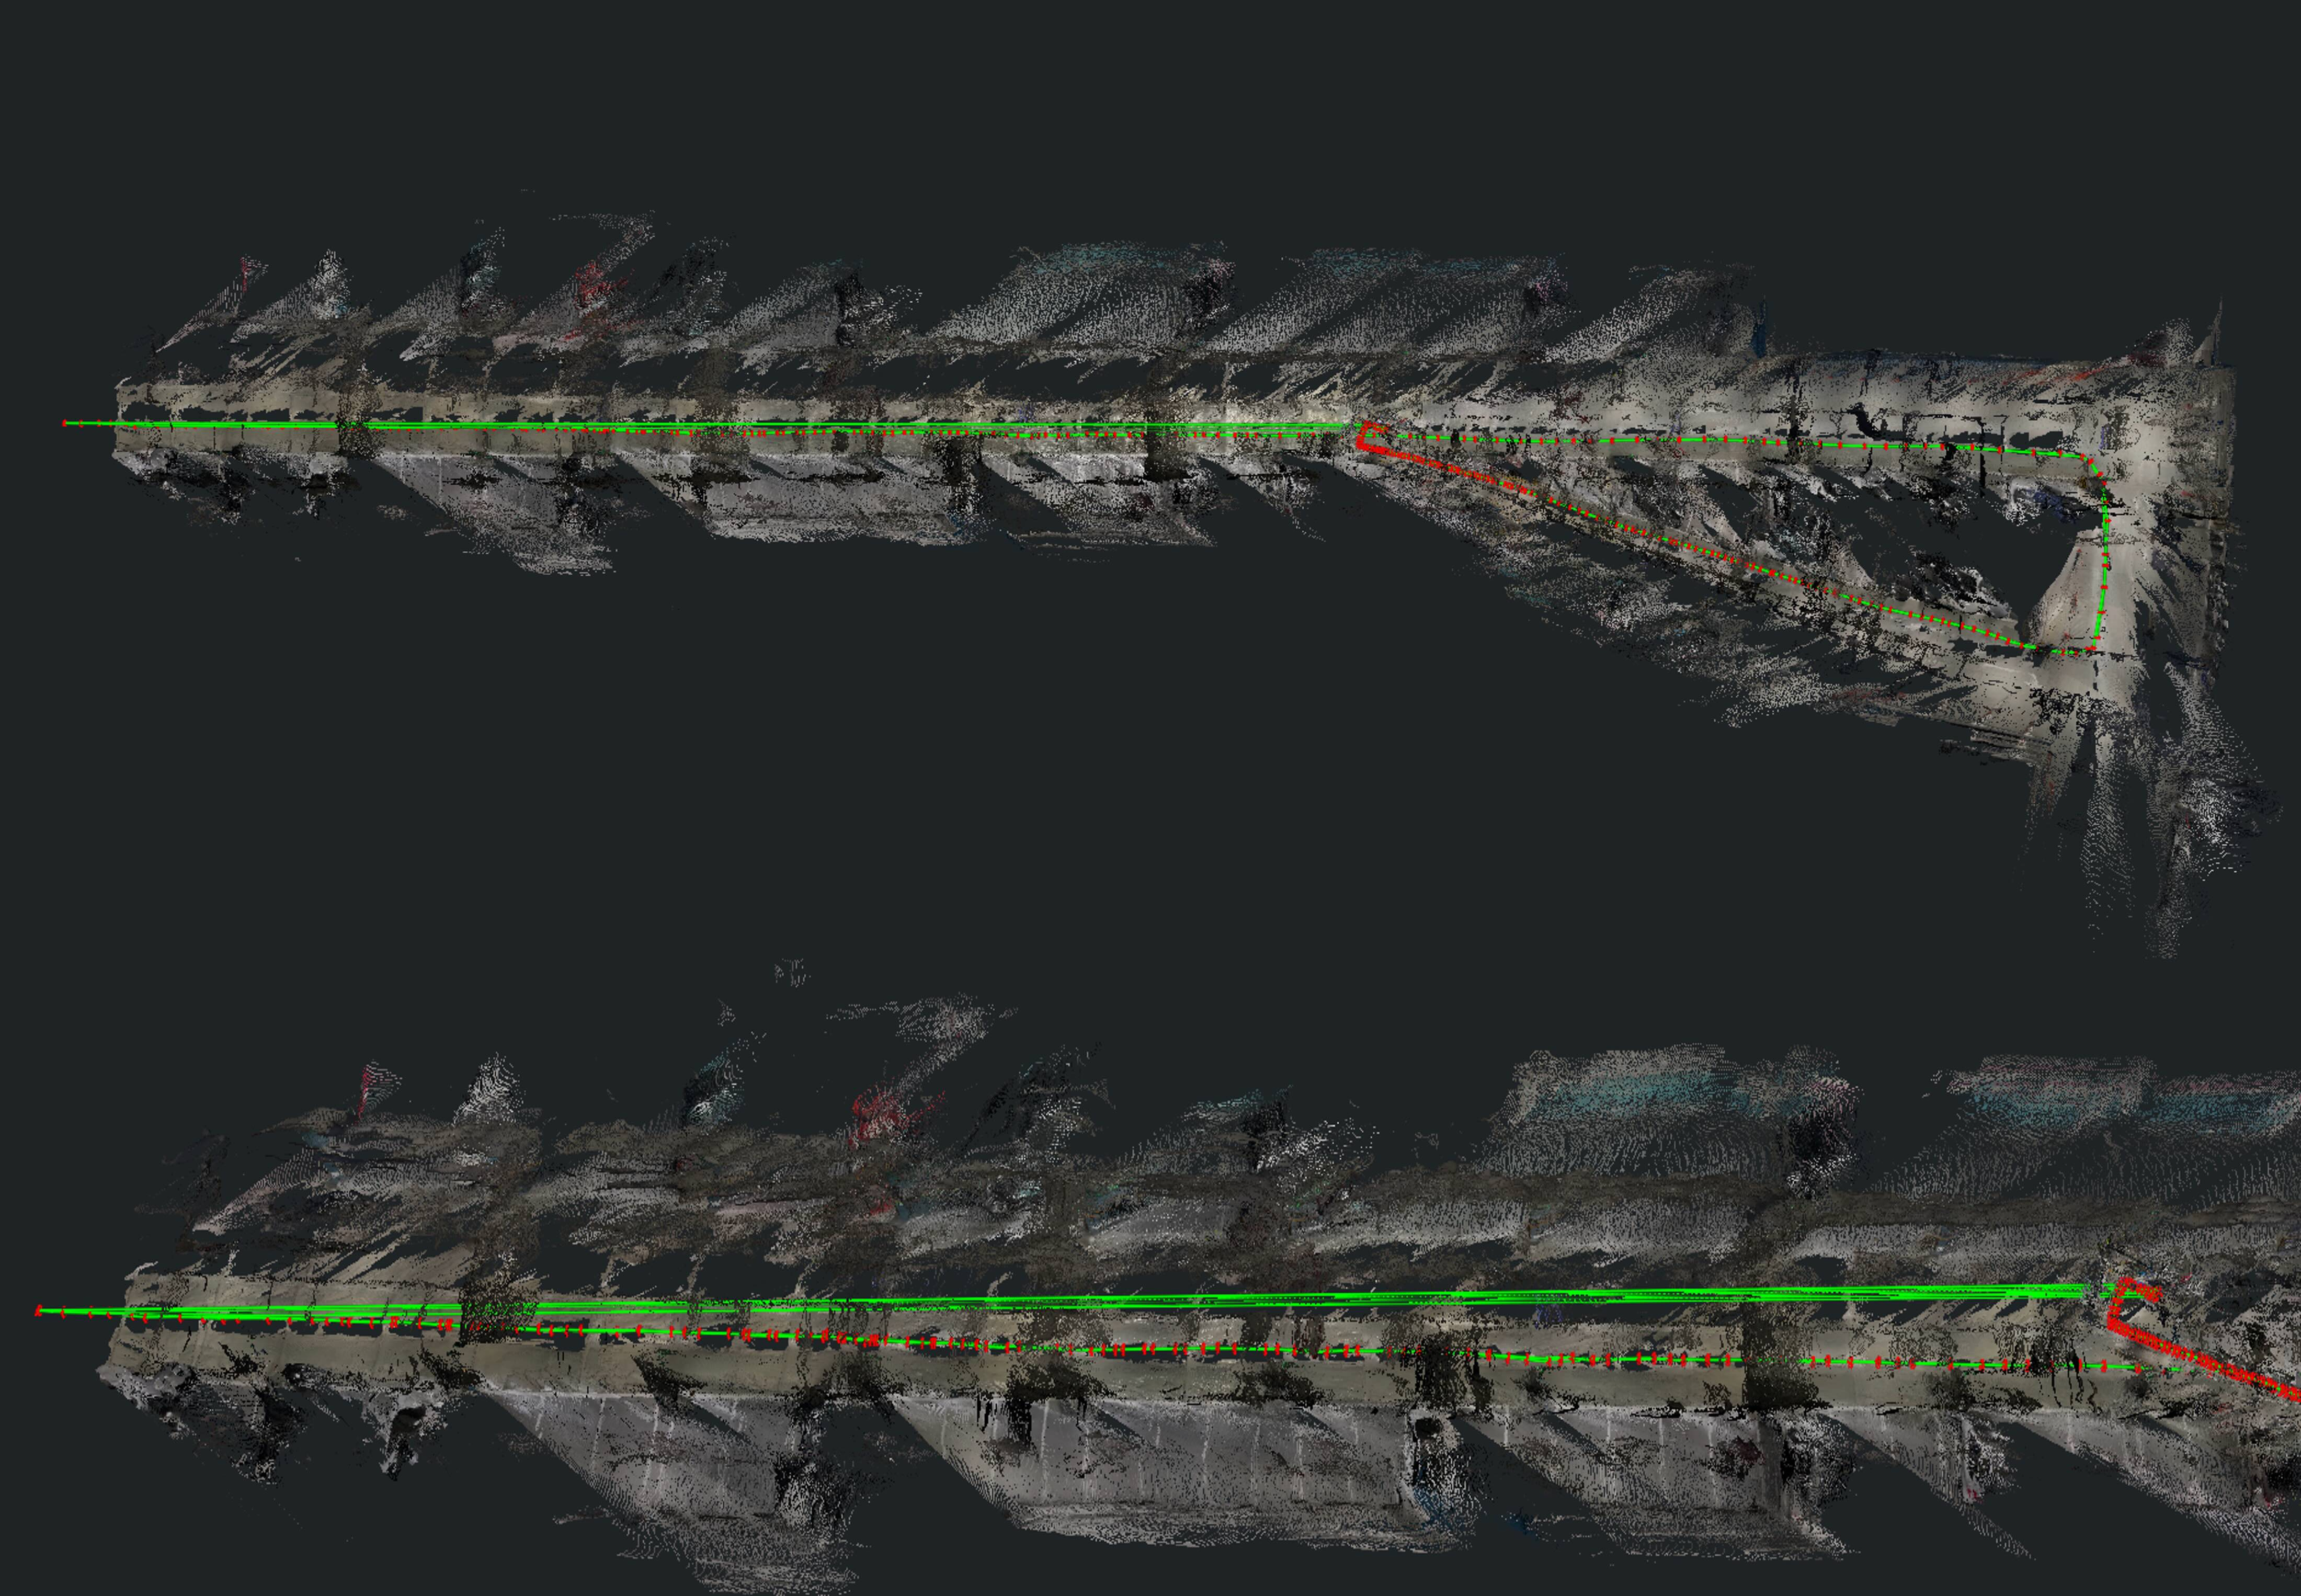
\includegraphics[width=0.98\columnwidth]{fig/long_term_7.jpg}
      \begin{overpic}[width=0.95\linewidth]{fig/long_term_7.jpg}
        \put(1,66){\color{white}\scriptsize Actual trajectory returns to origin but Sim(3) drift accumulates}
        \put(1,30){\color{white}\scriptsize Loop closure detected but Sim(3) optimization fails}
      \end{overpic}
        
    % \caption{A long-term optimization failure case for MASt3R-SLAM on the \texttt{Parking\_B2\_Loop} sequence. Despite successful loop detection, a geometrically distorted map was generated as the global optimization failed to correct for the massive scale drift accumulated over hundreds of meters. TODO}
    \caption{A long-term optimization failure case for MASt3R-SLAM on the \texttt{Parking\_01} sequence.}

    % \vspace{-3mm}

    \label{fig:long_term_7}

\end{figure}
% 

% 
\begin{figure}[!t]
    \centering
    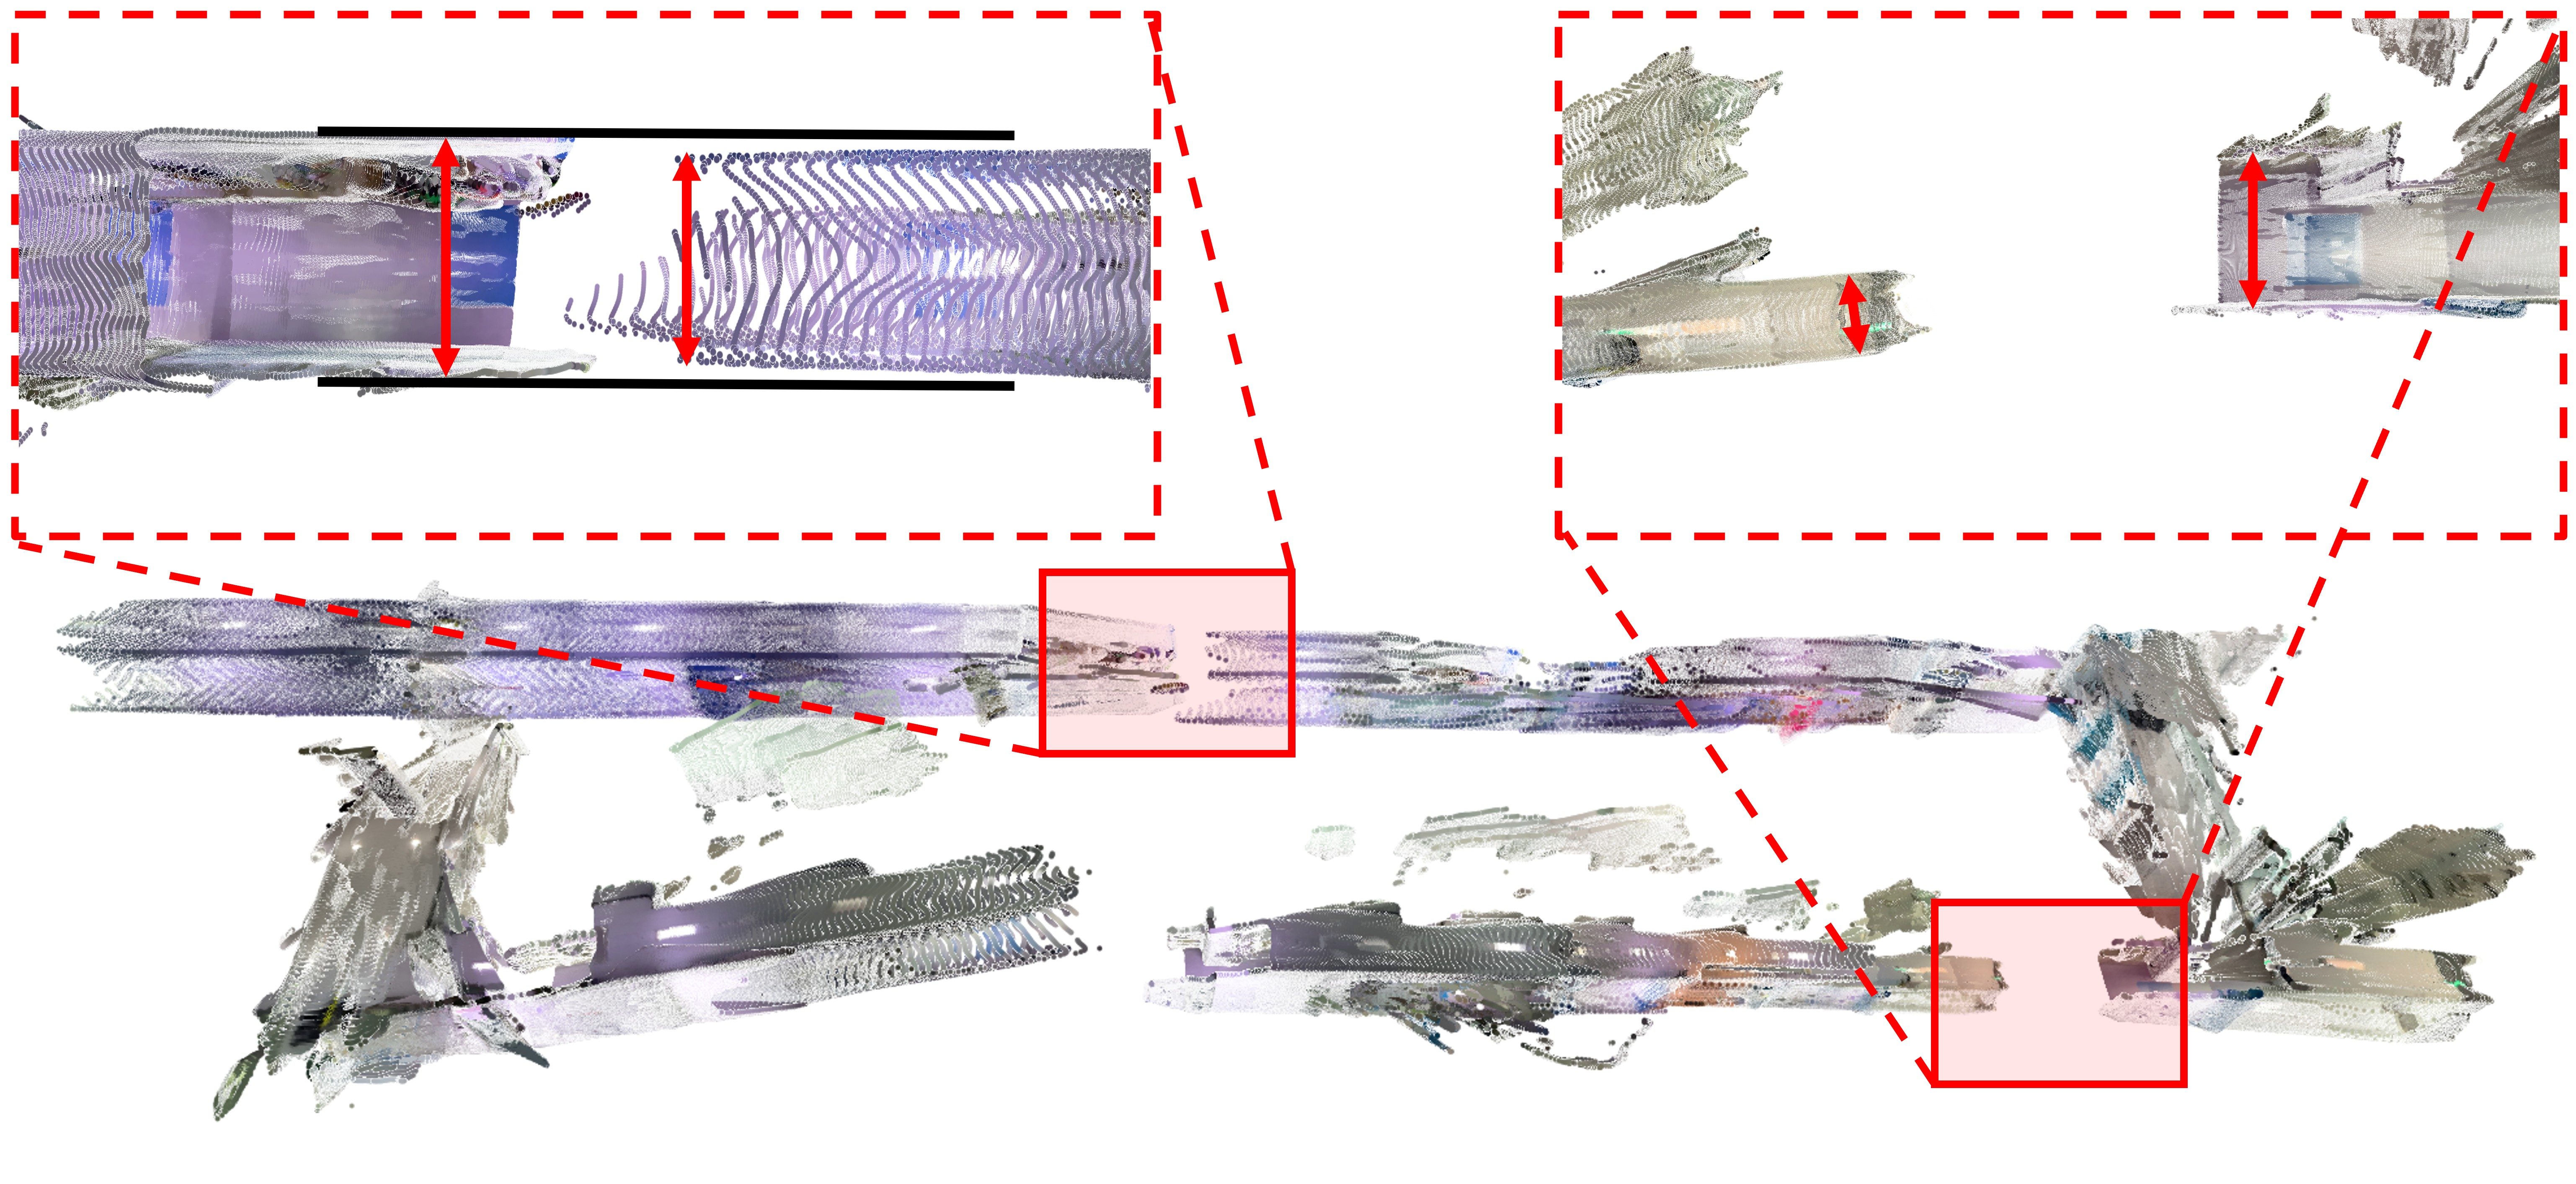
\includegraphics[width=1.0\columnwidth]{fig/fig7_v5.jpg}
    \caption{A failure case of inter-session scale ambiguity in MASt3R-SLAM. The image shows the result of processing a single sequence as three independent sessions. The resulting map fragments cannot be aligned into a consistent map as each was generated with a different, inconsistent scale.}

    \vspace{-3mm}

    \label{fig:multi_scale_inconsistency}
\end{figure}
% 
